%begin{figure}[!h]
%\begin{minipage}{.5\textwidth}
 % \centering
  %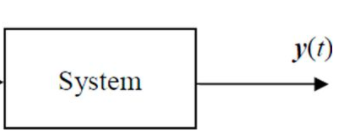
\includegraphics[width=.7\linewidth]{ts_system}
%\end{minipage}%
 % \begin{minipage}{.5\textwidth}
  %\centering
  %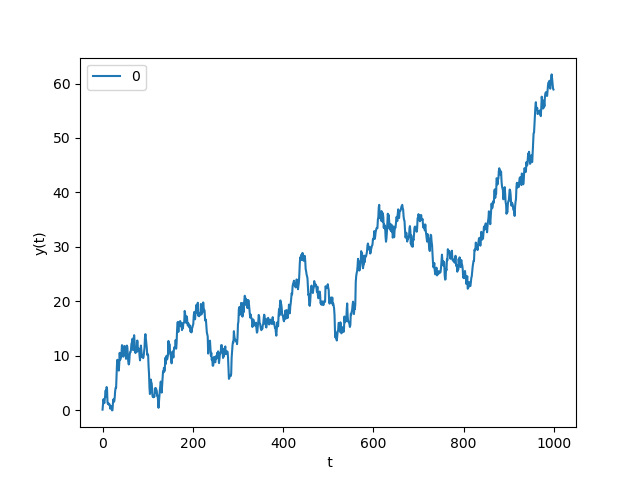
\includegraphics[width=.7\linewidth]{ts}
%\end{minipage}%
%\end{figure}
\section{Chapter 1 : Model classes}
\begin{figure}[!h]
  \centering
  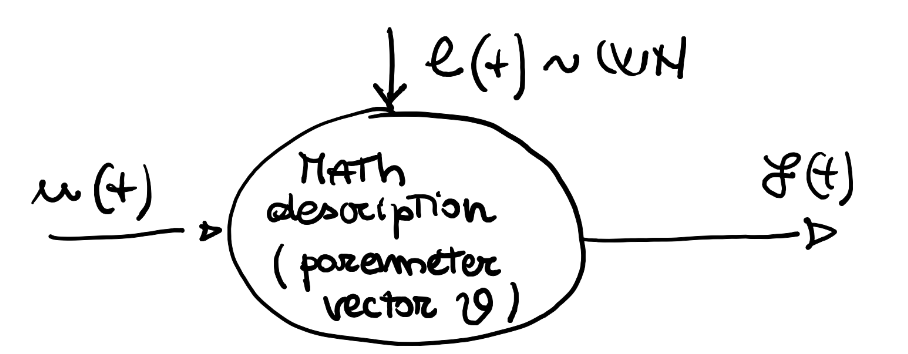
\includegraphics[width=.5\linewidth]{modelclasses}
\end{figure}
\[ \text{Mathematical model} =
\begin{cases}
	u(t) & \quad \text{input (I/O only)}\\
	e(t) & \quad \text{white noise}\\
	y(t) & \quad \text{output}
\end{cases}
\]
The mathematical model is described by \textbf{parametric parameter vector $\theta$ }that is found using a \textbf{parametric supervised} identification approach.\\
The models can be described with:
\begin{itemize}
\item \textbf{Differential Equations} in time domain
\item \textbf{Transfer functions}
\end{itemize}
%---------------------------------------------------------------------------------------
\subsection{Time-Series model classes}
The following processes are modelled with \textbf{differential equations}
\subsubsection{Moving Average Models (MA)}
A process y(t) \textbf{generated} by a WN e(t) is a moving average of order n   
 \textbf{MA(n)} process if: 
$$ y(t) = c_0e(t)+c_1e(t-1)+...+c_ne(t-n)$$ 
with parameter vector $ \theta = \{c_0 ,...,c_n\}$
\newpage
\begin{figure}[!ht]
  \centering
  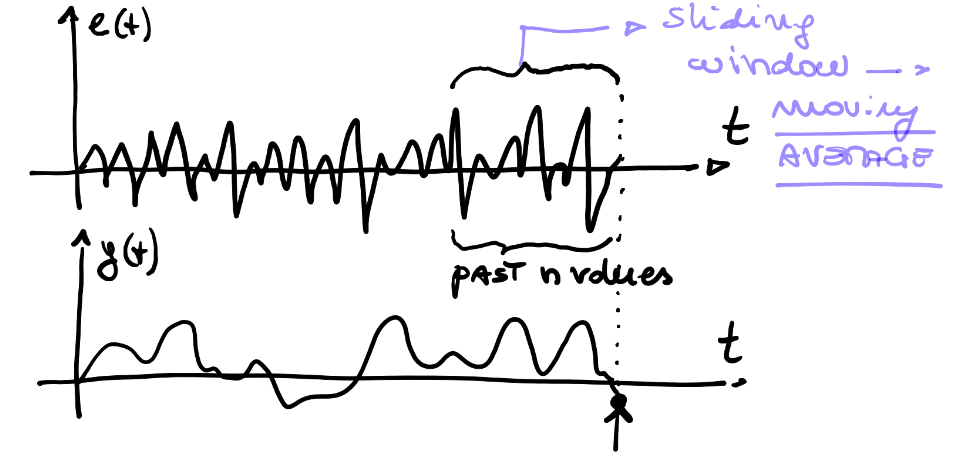
\includegraphics[width=.7\linewidth]{movingavg}
  \caption{y(t) is linear combination of past n e(t) values}
\end{figure}
\subsubsection{Autoregressive Models (AR)}
A process y(t) \textbf{generated} by a WN e(t) is an autoregressive of order m \textbf{AR(m)} process if:
$$ y(t) = a_1y(t-1)+a_2y(t-2)+...+a_my(t-m)+c_0e(t)$$ 
with parameter vector $ \theta = \{c_0,a_1,...,a_m\}$
\subsubsection{Autoregressive Moving Average Models (ARMA)}
A process y(t) \textbf{generated} by a WN e(t) is an ARMA of order (n,m) \textbf{ARMA(n,m)} process if:
$$ y(t) = a_1y(t-1)+a_2y(t-2)+...+a_my(t-m)+ c_0e(t)+c_1e(t-1)+...+c_ne(t-n)$$ 
with parameter vector $ \theta = \{c_0 ,...,c_n,a_1,...,a_m\}$\\
ARMA(0,n) $\to$ MA(n) : MA(n) is \textbf{subclass} of ARMA\\
ARMA(m,0) $\to$ AR(m) : AR(m) is \textbf{subclass} of ARMA

%---------------------------------------------------------------------------------------
\newpage
\subsection{Input/Output model classes}
The following processes are modelled with \textbf{differential equations}

\subsubsection{Autoregressive Moving Average Exogenous (ARMAX)}
A process y(t) \textbf{generated} by a WN e(t) and \textbf{exogenous} signal u(t) is an ARMAX of order (n,m, p+k) process if:
$$ y(t) = a_1y(t-1)+...+a_my(t-m)+ c_0e(t)+...+c_ne(t-n)+ b_0u(t-k)+...+b_pu(t-k-p)$$ 
with parameter vector $ \theta = \{c_0 ,...,c_n,a_1,...,a_m,b_0,...,b_p\}$\\
$ K \geq 1$ plays an important role : it represents the pure/intrinsic \textbf{delay} between y(t) and u(t).
\begin{figure}[!h]
  \centering
  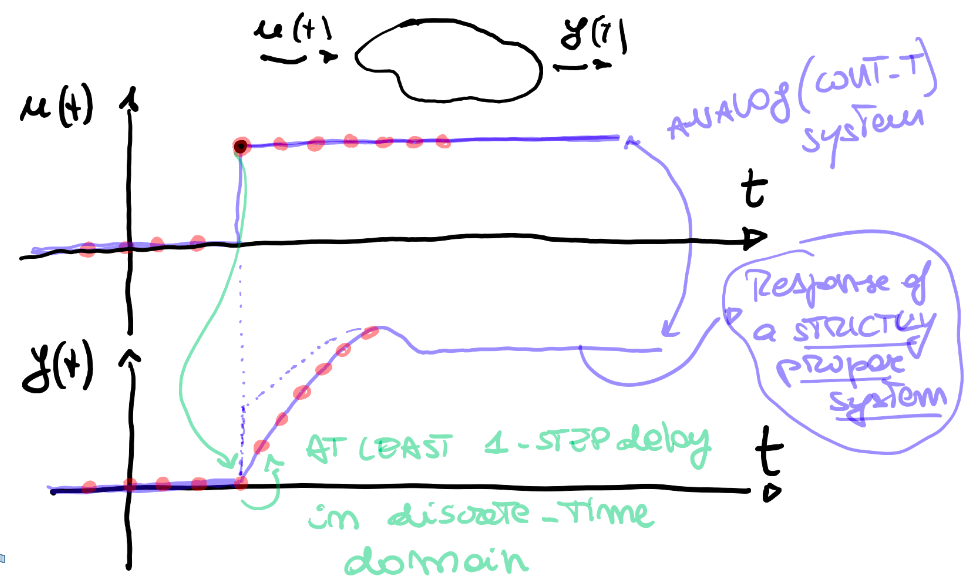
\includegraphics[width=.7\linewidth]{armax}
\end{figure}
If u(t) is a step the corresponding output y(t) is shown in figure.\\
Sampling (red dots) gives a discrete approximation : when the input slope rises a sample is taken resulting in a high value. The corresponding output is still low : this causes a \textbf{1 step delay}
\begin{description}
\item[Example]\hfill\\
$ y(t)=\frac{1}{2}y(t-1)+\frac{1}{3}y(t-2)+e(t)+e(t-3)+u(t-2)+\frac{1}{2}u(t-4) $
The process is an ARMAX (2,3,2+2)\\
Observation : missing values as above can be present!
\newpage
\par\noindent\rule{\textwidth}{0.4pt}
\item[Remark]\hfill\\
Armax models are the most general class models for \textbf{dynamic ,linear, time-invariant} systems.\\
\textbf{Non-Linear} N-ARMAX $ y(t) = f(y(t-1),..,y(t-m),e(t),...,e(t-n),u(t-k),...,u(t-k-p)$ \\ depend on \textbf{non-linear functions} : polynomials , splines ,NN ,Radial Basis Functions ,Fuzzy Sets.
\par\noindent\rule{\textwidth}{0.4pt}
\end{description}


\subsection{Transfer function representation}
The four models found above can be represented using \textbf{transfer functions}.
To transform time domain equations into the equivalent transfer function representation the \textbf{Z operator} is introduced.
\subsubsection{Z Operator}
\begin{itemize}
\item The operator $ Z^{-1}$ is the \textbf{backward shift} operator : $$ Z^{-1}x(t) = x(t-1)$$
\item The operator $ Z^{+1}$ is the \textbf{forward shift} operator : $$ Z^{+1}x(t) = x(t+1)$$
\end{itemize}
Both operators have properties : 
\begin{itemize}
\item \textbf{Linearity} : $ Z^{-1}(ax(t)+by(t)) = Z^{-1}ax(t)+Z^{-1}by(t) = ax(t-1)+by(t-1)$
\item \textbf{Recursion} : $ Z^{-1}(Z^{-1}...(Z^{-1}x(t))) = x(t-n) =Z^{-n} $ 
\end{itemize}


\subsubsection{Time domain to Transfer Function}
The Z operators are used to shift the equations of the time domain to be all at time \textbf{t}.\\
In case of a generic \textbf{ARMAX(m,n,p+k)} process 
$$ y(t) = a_1y(t-1)+...+a_my(t-m)+c_0e(t)+...+c_ne(t-n)+b_0u(t-k)+...+b_pu(t-k-p)$$
Applying the $Z^{-1}$ operator:
$$ y(t) = a_1Z^{-1}y(t)+...+a_mZ^{-m}y(t)+c_0e(t)+...+c_nZ^{-n}e(t)+b_0Z^{-k}u(t)+...+b_pZ^{-k-p}u(t)$$
Collecting :
$$ y(t)[1-a_1Z^{-1}+...+a_mZ^{-m}] =[c_0e+...+c_nZ^{-n}]e(t)+[b_0Z^{-k}+...+b_pZ^{-k-p}]u(t)$$
Dividing :
$$ y(t)=\frac{[c_0e+...+c_nZ^{-n}]}{[1-a_1Z^{-1}+...+a_mZ^{-m}]}e(t)+ \frac{[b_0+...+b_pZ^{-p}]}{[1-a_1Z^{-1}+...+a_mZ^{-m}]}u(t)Z^{-k}$$
Defining :
$$ A(Z) = 1-a_1Z^{-1}+...+a_mZ^{-m} $$
$$ B(Z) = b_0+...+b_pZ^{-p} $$
$$ C(Z) = c_0e+...+c_nZ^{-n} $$ 
The resulting process using TF representation is :
$$ y(t) = \frac{C(Z)}{A(Z)}e(t) + \frac{B(Z)}{A(Z)}u(t)Z^{-k} $$
\begin{figure}[!h]
\begin{minipage}{.5\textwidth}
 \centering
  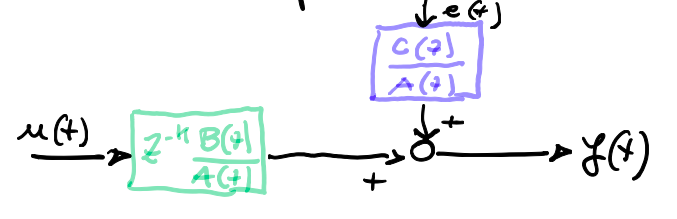
\includegraphics[width=.7\linewidth]{blockio}
\end{minipage}%
	\begin{minipage}{.5\textwidth}
  \centering
  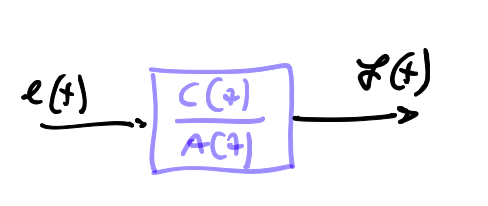
\includegraphics[width=.55\linewidth]{blockts}
\end{minipage}%
\end{figure}

\subsubsection{From $Z^{-}$ to $Z^{+}$ }
The transfer functions can be written in negative, positive o mixed power of Z.
The example explains how to get the positive power representation starting from a negative one :
$$ y(t)= \frac{c_0+c_1Z^{-1}+...+c_nZ^{n}}{1-a_1Z^{-1}-...-a_mZ^{-m}} e(t)$$
If $ m \geq n $ by multiplying by $Z^{+m}$ : 
$$ y(t)= \frac{c_0Z^m+c_1Z^{m-1}+...+c_nZ^{m-n}}{Z^m-a_1Z^{m-1}-...-a_m} e(t)$$
\begin{description}
\item[Observation]\hfill\\
Even if feasible and correct it is better to \textbf{avoid} the mixed representation!
\end{description}
\newpage
\subsubsection{Importance of stationary property}
Transformation \textbf{Time Domain} $ \leftrightarrow $ \textbf{Transfer Functions} are \textbf{feasible} if the \textbf{stationary property} holds because otherwise the Z operator is not applicable.\\
$$ y(t) = \frac{Z+\frac{1}{2}}{Z-\frac{1}{3}}e(t) , \text{e(t) - WN(0,1)} $$
\begin{description}
\item[In time domain]\hfill\\
$$(Z-\frac{1}{3})y(t) = (Z+\frac{1}{2})e(t) $$
$$ y(t+1)-\frac{1}{3}y(t) = e(t+1)+\frac{1}{2}e(t) $$
$$y(t+1) = \frac{1}{3}y(t) + e(t+1)+\frac{1}{2}e(t) $$
Time shift to start a time "t" ( can be done in stationary conditions):
$$y(t) = \frac{1}{3}y(t-1) + e(t)+\frac{1}{2}e(t-1) $$
\item[Back to TF]\hfill\\
$$y(t) = \frac{1}{3}Z^{-1}y(t) + e(t)+\frac{1}{2}Z^{-1}e(t) $$
$$[1-\frac{1}{3}Z^{-1}]y(t) = [1+\frac{1}{2}Z^{-1}]e(t) $$
$$y(t) = \frac{[1+\frac{1}{2}Z^{-1}]}{[1-\frac{1}{3}Z^{-1}]} e(t) $$
\end{description}

\newpage
\subsubsection{Pole,Zeros and Stability}
\begin{figure}[!h]
 \centering
  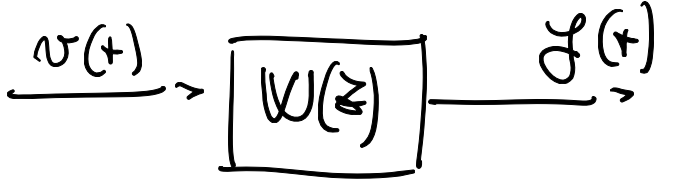
\includegraphics[width=.4\linewidth]{wnsys}
\end{figure}
Considering a process with signals e(t) , y(t) and a system W(Z) represented in \textbf{positive/null} power: 
\begin{itemize}
\item \textbf{Poles} of W(Z) are the \textbf{roots} of the denominator
\item \textbf{Zeros} of W(Z) are the \textbf{roots} of the nominator
\end{itemize}
A system is said to be \textbf{asymptotically stable} if and only if all the \textbf{poles} of W(Z) are \textbf{strictly inside} the unit circle (left graph).\\
Blue = unstable region \\
Red = simple stability region \\
Green = asymptotically stability region \\
\begin{figure}[H]
\begin{minipage}{.5\textwidth}
 \centering
  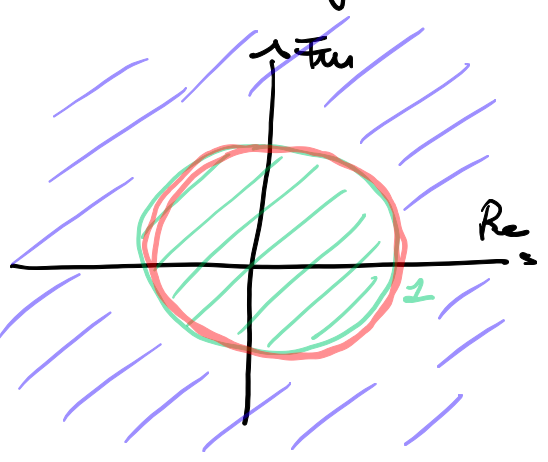
\includegraphics[width=.7\linewidth]{disstab}
\end{minipage}%
	\begin{minipage}{.5\textwidth}
  \centering
  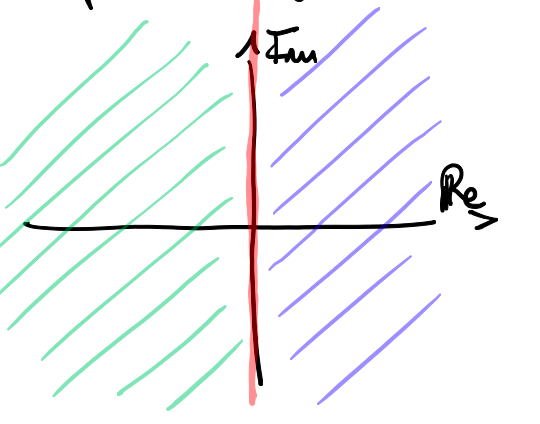
\includegraphics[width=.7\linewidth]{contstab}
\end{minipage}%
\end{figure}
\textbf{Note:} if we were dealing with \textbf{continuous} signals and processes instead of Z transformation we would apply \textbf{Laplace} . Also the stability region would change as seen on the right graph.
\newpage
\begin{description}
\item[Example:]\hfill\\
$$ W(Z) = \frac{1-\frac{1}{2}Z^{-1}}{1+\frac{1}{3}Z^{-1}} $$ 
Move to positive power:
$$ W(Z) = \frac{Z-\frac{1}{2}}{Z+\frac{1}{3}} $$ 
\begin{itemize}
\item \textbf{Pole} : $ Z = -\frac{1}{3} $
\item \textbf{Zero} : $ Z = \frac{1}{2} $
\end{itemize}
\begin{figure}[!h]
 \centering
  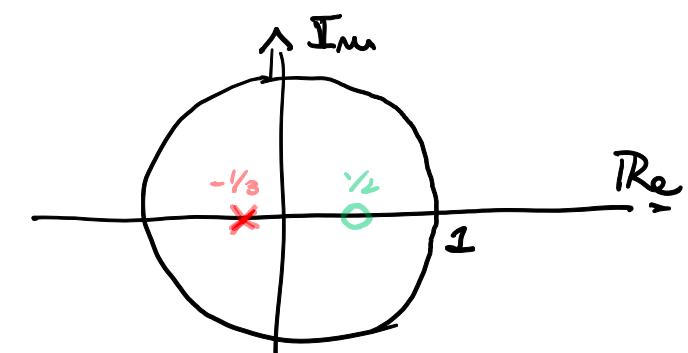
\includegraphics[width=.4\linewidth]{stabex}
\end{figure}
The system is asymptotically stable since all poles are within the unit circle.
\end{description}

\subsubsection{Stationary property and stability }
\begin{figure}[!h]
 \centering
  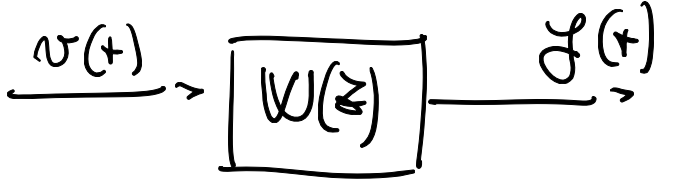
\includegraphics[width=.4\linewidth]{wnsys}
\end{figure}
In a stochastic process y(t) obtained as output of a system W(Z) fed with a stochastic process v(t) , y(t) is a \textbf{stationary process SSP} if and only if:
\begin{enumerate}
\item v(t) is a \textbf{stationary stochastic process}
\item W(Z) is \textbf{asymptotically stable}
\end{enumerate}
Checking the stationary property is usually very long , instead these two properties make it easy : input v(t) is usually a \textbf{white noise} which is a \textbf{stationary stochastic process}.
\subsubsection{Poles and Zeros in MA \& AR processes}
\begin{description}
\item[ MA(1)]\hfill\\
$$ y(t) = e(t) + \frac{1}{2}e(t-1)$$
$$ y(t) = (1+\frac{1}{2} Z^{-1})e(t) $$
$$ y(t) = (\frac{Z+\frac{1}{2}}{Z})e(t) $$
\begin{itemize}
\item \textbf{Zero} : $ Z= -\frac{1}{2}$
\item \textbf{Pole} : $ Z= 0 $
\end{itemize}
\item[AR(1)]\hfill\\
$$ y(t) = \frac{1}{2}y(t-1)+3e(t)$$
$$ y(t) = (\frac{3Z}{Z-\frac{1}{2}})e(t) $$
\begin{itemize}
\item \textbf{Zero} : $ Z= 0$
\item \textbf{Pole} : $ Z= \frac{1}{2}$
\end{itemize}
\item[General conclusion]\hfill\\
A \textbf{MA(n)} process is generated by a TF having :
\begin{itemize}
\item n \textbf{generic} zeros
\item n poles \textbf{all in 0} $\to$ \textbf{always stationary!}
\end{itemize}
It is also called \textbf{All-Zeros} process \\
An \textbf{AR(m)} process i s generated by a TF having :
\begin{itemize}
\item m zero \textbf{all in 0}
\item m \textbf{generic} poles
It is also called \textbf{All-Poles} process
\end{itemize}
\end{description}

